\documentclass[11pt,a4paper]{article}
\usepackage[T1]{fontenc}
\usepackage[utf8]{inputenc}
\usepackage{amsmath,amsthm}
% Libertinus for text and math: lower stroke contrast than Computer Modern, so
% hairlines survive screen rasterization. Also avoids the autotraced cm-super
% fallback that CM pulls in for TS1 glyphs. libertinust1math supplies \mathbb,
% \mathcal and the operators, so amssymb is not loaded (it would clash).
\usepackage{libertinus}
\usepackage[libertine]{libertinust1math}
\usepackage{hyperref}
\usepackage{microtype}
\usepackage{booktabs}
\usepackage[margin=1in]{geometry}
\usepackage{enumitem}
\usepackage{xcolor}
\usepackage{tikz}
\usetikzlibrary{arrows.meta,positioning}

\hypersetup{colorlinks=true,linkcolor=blue!50!black,urlcolor=blue!50!black}

\newcommand{\lean}[1]{\texttt{#1}}
\newcommand{\Vplus}{V_{+}}

\title{What the Verified OS Reconstruction Package Proves\\
{\large and what it does not}}
\author{Status note}
\date{26 September 2026 \\[2pt]
{\small \lean{xiyin137/OSreconstruction}, \lean{main} at \lean{32feb1f5}}}

\begin{document}
\maketitle

\begin{abstract}
The repository contains a machine-checked, axiom-free proof of the
Osterwalder--Schrader correspondence in \emph{both} directions, for every
spatial dimension $d \ge 1$. It is nevertheless \emph{not} a proof that the
Euclidean and Wightman axioms are equivalent. The Euclidean-to-relativistic
direction consumes a growth hypothesis that the reverse direction does not
produce, so the two implications do not compose into a biconditional; and
``Wightman'' here means the Wightman \emph{functions}, not the operator theory.
This note states the three proved theorems exactly, and isolates every
qualification attached to them. All line references are to
\lean{os-reconstruction/verification/comparator/Definitions.lean}.
\end{abstract}

\section{What is in the repository}

Two independent Lean trees currently sit side by side on \lean{main}.

\begin{center}
\begin{tabular}{@{}llll@{}}
\toprule
Tree & \lean{.lean} files & Status & Provenance \\
\midrule
\lean{os-reconstruction/} & 854 & the verified package & PR \#93, \#94, \#95, \#96, \#97 \\
\lean{OSReconstruction/} (root) & 361 & superseded development tree & pre-\#93 history \\
\bottomrule
\end{tabular}
\end{center}

Only the first is the subject of this note. The root tree still states a
growth clause that was refuted by explicit counterexample, and nothing in it is
marked deprecated; PR \#98 removes it, and is open awaiting review. Until that
lands, a reader can pick up a refuted statement from the repository root by
accident.

The package pins Lean and Mathlib \lean{v4.33.0-rc1} and depends on exactly one
project library, \lean{gaussian-field} at \lean{f2481cf}. The \lean{hille-yosida},
\lean{bochner} and \lean{kolmogorov\_extension4} dependencies were dropped in \#95.

\section{The verification boundary}

The package carries its own external audit surface, \lean{verification/comparator/}:

\begin{description}[leftmargin=2.2em,itemsep=2pt]
\item[\lean{Definitions.lean}] 493 lines importing \emph{only} Mathlib. Every
project-specific notion used by the three propositions is defined here from
scratch. This is the single file a reader must audit to know what was proved.
\item[\lean{Challenge.lean}] states the three propositions as named obligations,
with \lean{sorry} placeholders. These are the only \lean{sorry}s anywhere in the
package. Nothing imports this module, and the placeholders never enter the
solution environment.
\item[\lean{Solution.lean}] proves the same three named theorems from the
production library via \lean{Main.lean}, through bridge equivalences
(\lean{eToR\_iff}, \lean{eToROSII\_iff}, \lean{rToE\_iff}) that identify the
independent audit statements with the production ones.
\end{description}

The permitted axiom whitelist in \lean{comparator.json} is
\[
  \{\ \lean{propext},\quad \lean{Quot.sound},\quad \lean{Classical.choice}\ \}.
\]
That is, the standard classical foundations and nothing else: no project axioms.
A source scan over the package finds no \lean{axiom} declarations and no
\lean{sorry} outside \lean{Challenge.lean}.

\section{The objects}

Spacetime has dimension $d+1$ with $d \ge 1$ (the \lean{NeZero d} hypothesis);
$1$-dimensional spacetime is excluded. Write
\[
  \text{Point } d = \mathbb{R}^{d+1}, \qquad
  \text{Test } d\, n = \mathcal{S}\big((\mathbb{R}^{d+1})^{n};\mathbb{C}\big), \qquad
  \text{Family } d = \textstyle\prod_{n} \big(\text{Test } d\, n \to \mathbb{C}\big).
\]

\paragraph{The Euclidean side.}
\lean{OS d} (line 300) is a Schwinger family
$S_n$ defined on the \emph{zero-diagonal} test space $^{\circ}\mathcal{S}$
(\lean{ZeroTest}, line 256): Schwartz functions all of whose derivatives vanish on
every coincidence locus $x_i = x_j$, $i \ne j$. The fields are exactly
E0 (temperedness, linearity, reality), E1 (translation and $SO(d+1)$ rotation
invariance), E2 (reflection positivity), E3 (permutation symmetry) and
E4 (clustering). Stating the axioms on $^{\circ}\mathcal{S}$ rather than on full
Schwartz space is deliberate: inverse-power coincidence singularities of finite
order are compatible with $^{\circ}\mathcal{S}$, and the passage from
$^{\circ}\mathcal{S}$ to genuine tempered Wightman distributions is the
substance of the theorem.

\paragraph{The relativistic side.}
\lean{Wightman d} (line 194) is a family $W_n$ together with linearity,
temperedness, normalization $W_0(f) = f(0)$, translation invariance, covariance
under the connected Lorentz group, the spectrum condition
(\lean{forwardAnalyticity}), a spectral support condition, adjacent locality,
positive-definiteness, Hermiticity, and clustering.

\paragraph{The pairing.}
\lean{wickPair} (line 350) is the link between the two sides: for each $n$ there is
a single holomorphic $F$ on the forward tube whose distributional boundary values
along forward directions give $W_n$, and whose restriction to Wick-rotated
Euclidean points, $x \mapsto (ix^0, \vec{x}\,)$, integrates against
zero-diagonal tests to give $S_n$. One kernel, both families.

\paragraph{The growth conditions.}
Two are defined. \lean{arityLinearGrowth} (line 336) asks
\[
  \|S_n(f)\| \;\le\; \alpha\,\beta^{n}\,(n!)^{\gamma}\;
  \|f\|_{\text{arity-linear seminorm}},
\]
with the Schwartz seminorm order growing linearly in the arity $n$.
\lean{originalGrowth} (line 393) is the OS II (4.1) variant in original
coordinates, with strictly positive Sobolev index and a factorial-only prefactor.
\lean{outputGrowth} (line 405) is the OS II (4.3) conclusion on the Wightman side.

\section{The three theorems}

\begin{enumerate}[leftmargin=2.4em,itemsep=6pt]
\item \textbf{E$'\to$R} (\lean{EToR}, line 475):
\[
  \forall A : \lean{OS}\ d,\quad
  \lean{arityLinearGrowth}\ A \;\longrightarrow\;
  \exists W : \lean{Wightman}\ d,\ \lean{wickPair}\ A.S\ W.W .
\]

\item \textbf{E$'\to$R$'$, OS II form} (\lean{EToROSII}, line 481):
\[
  \forall A : \lean{OS}\ d,\quad
  \lean{originalGrowth}\ A \;\longrightarrow\;
  \exists W,\ \lean{wickPair}\ A.S\ W.W \ \wedge\ \lean{outputGrowth}\ d\ W.W
  \ \wedge\ \big(\forall V,\ \lean{wickPair}\ A.S\ V \to V = W.W\big).
\]
This is the only one of the three that delivers \emph{uniqueness}: the Wightman
functions are determined by the Schwinger functions they Wick-pair with.

\item \textbf{R$\to$E} (\lean{RToE}, line 489):
\[
  \forall W : \lean{Wightman}\ d,\quad
  \exists A : \lean{OS}\ d,\
  A.S = \lean{constructSchwinger}\ W \ \wedge\ \lean{wickPair}\ A.S\ W.W .
\]
Note two strengths here: there is \emph{no} growth hypothesis, and the Schwinger
family is not merely asserted to exist but is pinned to a fixed, explicitly
defined constructor (line 465), so the reverse direction is canonical rather than
existential.
\end{enumerate}

\section{The logical shape, and why it is not an equivalence}

Combining the directions, what is proved is
\[
  \boxed{\ \text{OS axioms} \;+\; \text{growth}
  \quad\Longrightarrow\quad \text{Wightman}
  \quad\Longrightarrow\quad \text{OS axioms}\ }
\]
with the growth hypothesis present on the left arrow and absent from the right.

\begin{center}
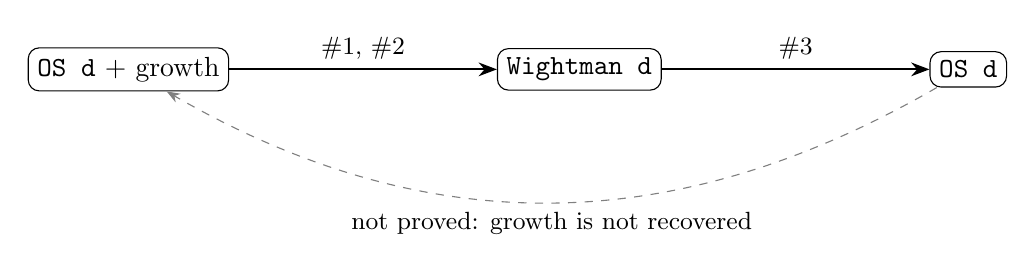
\begin{tikzpicture}[>=Stealth,node distance=16mm and 34mm]
  \node[draw,rounded corners,align=center] (osg) {\lean{OS d} $+$ growth};
  \node[draw,rounded corners,align=center,right=of osg] (w) {\lean{Wightman d}};
  \node[draw,rounded corners,align=center,right=of w] (os) {\lean{OS d}};
  \draw[->,thick] (osg) -- node[above,font=\small] {\#1, \#2} (w);
  \draw[->,thick] (w) -- node[above,font=\small] {\#3} (os);
  \draw[->,dashed,gray] (os) to[out=-150,in=-30] node[below,font=\small,black] {not proved: growth is not recovered} (osg);
\end{tikzpicture}
\end{center}

Consequently:

\begin{itemize}[leftmargin=1.6em,itemsep=4pt]
\item \textbf{Sufficiency is proved.} The Euclidean axioms together with a growth
condition suffice to produce a Wightman theory.
\item \textbf{Necessity is proved only for the axioms, not for the growth
condition.} Every Wightman theory yields the OS axioms, but nothing here shows
that the Schwinger functions so obtained satisfy \lean{arityLinearGrowth} or
\lean{originalGrowth}. There is a genuine gap between the sufficient condition
and the necessary one.
\item \textbf{The round trip does not close.} Because R$\to$E produces no growth
data, its output cannot be fed back into E$\to$R. There is no proved
$\text{Wightman} \to \text{OS} \to \text{Wightman}$ identity. Nor is there a
proved $\text{OS} \to \text{Wightman} \to \text{OS}$ returning the \emph{same}
Schwinger family: R$\to$E pins its output to \lean{constructSchwinger}, which is
a different normalization from an arbitrary starting $A$.
\end{itemize}

This asymmetry is not an artifact of the formalization. It is the OS I $\to$
OS II correction itself: the original Osterwalder--Schrader axioms were not
sufficient, and the linear growth condition was introduced precisely to repair
the forward direction. The formalization reproduces that state of affairs
faithfully, including its incompleteness.

\section{Four further qualifications}

\paragraph{1. ``Wightman'' means the Wightman functions, not the operator theory.}
\lean{Wightman d} is a family of tempered distributions satisfying the Wightman
\emph{function} axioms. There is no Hilbert space, no unitary representation of
the Poincar\'e group, no field operators and no vacuum vector in any of the three
statements. The reconstruction of an operator theory from such a family is a
separate classical theorem (GNS plus spectral theory); the production library
contains machinery for it, but it is not what the audited theorems assert.

\paragraph{2. The forward tube is smaller than the literal one.}
\lean{forwardTube} (line 76) requires, in addition to the successive-difference
conditions $\operatorname{Im}(z_k - z_{k-1}) \in \Vplus$ for $1 \le k < n$, the
absolute condition $\operatorname{Im} z_0 \in \Vplus$. For $n > 0$ this is a
\emph{proper subset} of the usual $n$-point forward tube, which is defined by the
difference conditions alone. The file says so explicitly (lines 70--75) and states
that \lean{forwardAnalyticity} and \lean{wickPair} ``do not assert extension to
the larger literal tube.'' Both the spectrum condition and the Wick pairing are
therefore weaker than their textbook counterparts.

\paragraph{3. Locality is the adjacent-transposition form.}
\lean{adjacentLocality} (line 90) asserts commutation only for neighbouring
labels $i, i+1$, on test functions supported where
$(x_i - x_{i+1})^2 > 0$. Adjacent transpositions generate $S_n$, so this is
plausibly equivalent to full locality in the presence of the remaining axioms,
but that equivalence is not part of the statement. Two open upstream PRs (\#84,
\#85) concern this API, so it should be treated as still moving.

\paragraph{4. E2's content rests on a totalization.}
\lean{osInnerProduct} (line 291) applies \lean{ZeroTest.ofClassical} to each
tensor witness, a total function that sends any test failing the zero-diagonal
condition to $0$. A product of two zero-diagonal tests need not vanish on
cross-block coincidences $x_i = x_j$ with $i$ in the first factor and $j$ in the
second, so precisely which terms of the reflection-positivity sum carry content
depends on that coercion. The docstring asserts that the correspondence proofs
establish non-vacuity; that claim has not been independently re-verified in
preparing this note.

\section{Where this leaves the project}

\begin{itemize}[leftmargin=1.6em,itemsep=4pt]
\item \textbf{Non-vacuity by instantiation} is the main outstanding mathematical
task. No model is yet exhibited that satisfies the hypotheses of E$\to$R. The
planned route is the Gaussian free field: build $n$-point Schwinger functions on
the zero-diagonal test space and verify E0--E4 together with a growth condition.
The package already depends on \lean{gaussian-field}, whose \lean{Wick.lean}
supplies integrability of products of field evaluations, the recursive
Isserlis/Wick identity, vanishing of odd moments, and the
$(n-1)!!\,$ and $\sqrt{n!}$ moment bounds --- the last of these being exactly the
shape the growth conditions demand. The missing step is a bridge identifying the
free-field measure with \lean{gaussian-field}'s Gaussian measure, after which
$S_n$ on $^{\circ}\mathcal{S}$ can be defined from the Wick kernel.
\item \textbf{Closing the gap} would mean either proving that a Wightman theory's
Schwinger functions satisfy a growth condition, or exhibiting a Wightman theory
whose Schwinger functions demonstrably do not. Either would turn the present
pair of implications into a sharp statement.
\item \textbf{Housekeeping:} PR \#98 (delete the superseded root tree) is open;
the forward-tube convention and the locality API are the two places where the
audited statements are weaker than the textbook ones and would repay
strengthening.
\end{itemize}

\vfill
\noindent\rule{\linewidth}{0.4pt}\\
{\small This note supersedes \lean{docs/os\_reconstruction\_status.md} (3 May 2026),
which describes the superseded root tree and its axiom and \lean{sorry} debts, not
the verified package.}

\end{document}
